\documentclass{article}
\usepackage{graphicx}
\usepackage[a4paper, margin=1in, top=0.5in]{geometry}  % Adjust top margin here

\title{Analysis Report: Age Assignment Model Comparison \\ Trust Stamp Assignment}
\author{Pablo Martínez-Agulló}
\date{September 2024}

\begin{document}

\maketitle

\section{Introduction}
Hanut, an online retailer, wants to enhance customer experiences by personalizing them based on age demographics. After exploring image-based age estimation solutions, they have shortlisted two models and are seeking our analysis to determine which model to adopt. Their consumer age profiles are segmented into specific brackets: 0-12, 13-15, 16-17, 18-24, 25-30, 31-40, 41-50, 51-60, 61-70, 71-80, and 81+.

The two shortlisted models are:
\begin{itemize}
    \item \textbf{Model 1}
    \begin{itemize}
        \item Predicts an age range, given as 'age\_min' and 'age\_max'.
        \item Data available in 'data/model\_1.csv', containing 6975 entries.
    \end{itemize}
    
    \item \textbf{Model 2}
    \begin{itemize}
        \item Provides a direct age prediction labeled as 'age'.
        \item Data available in 'data/model\_2.csv', containing 6969 entries.
    \end{itemize}
\end{itemize}

The actual age data is stored in 'data/gt.csv' with 8644 entries. Both models' datasets contain some missing entries when compared to the ground truth data. After merging the three datasets, the comparison is conducted on 6957 complete entries, with missing data removed.

\section{Data Exploration}

%\begin{table}[h]
%\centering
%\begin{tabular}{|c|c|c|c|c|}
%\hline
%\textbf{real\_age} & \textbf{model\_1\_age\_min} & \textbf{model\_1\_age\_max} & %\textbf{model\_2\_age} & \textbf{model\_1\_age\_avg} \\ \hline
%31.248095   & 27.082076   & 34.397298   & 30.985482   & 30.739687   \\ \hline
%\end{tabular}
%\caption{Mean values for real and predicted ages from Model 1 and Model 2.}
%\end{table}


On Figure~\ref{fig:Scatter} it can be already seen that as the real age goes higher, both models underestimate the age. The $R^2$ suggests a linear behavior, especially for Model 1. Note that on all plots, for the Model 1, the average between the 'age\_min' and 'age\_max'. 

The horizontal alignment of points for Model 2 (blue) indicates that its predictions might be discretized to specific values instead of providing more granular continuous predictions. The low $R^2$ score of Model 2 may be caused by this.



\begin{figure}[h]
    \centering
    \begin{minipage}{0.49\textwidth}
        \centering
        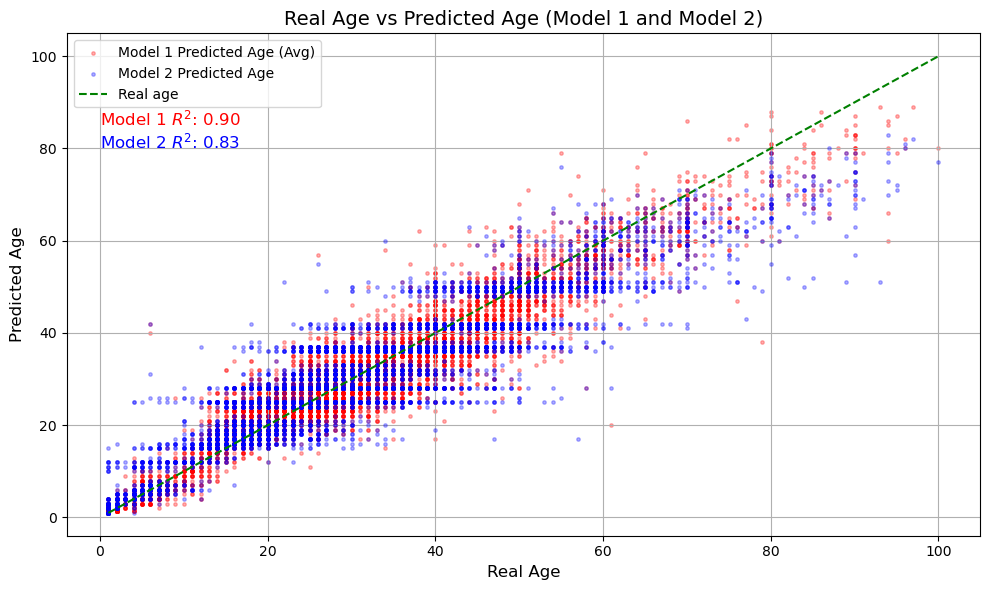
\includegraphics[width=\textwidth]{images/0_Scatter_Real_vs_prediction_Refined_dropNan_A.png}
        \caption{Scatter plot of predicted age for both models as a function of the real age.}
        \label{fig:Scatter}
    \end{minipage}
    \hfill
    \begin{minipage}{0.49\textwidth}
        \centering
        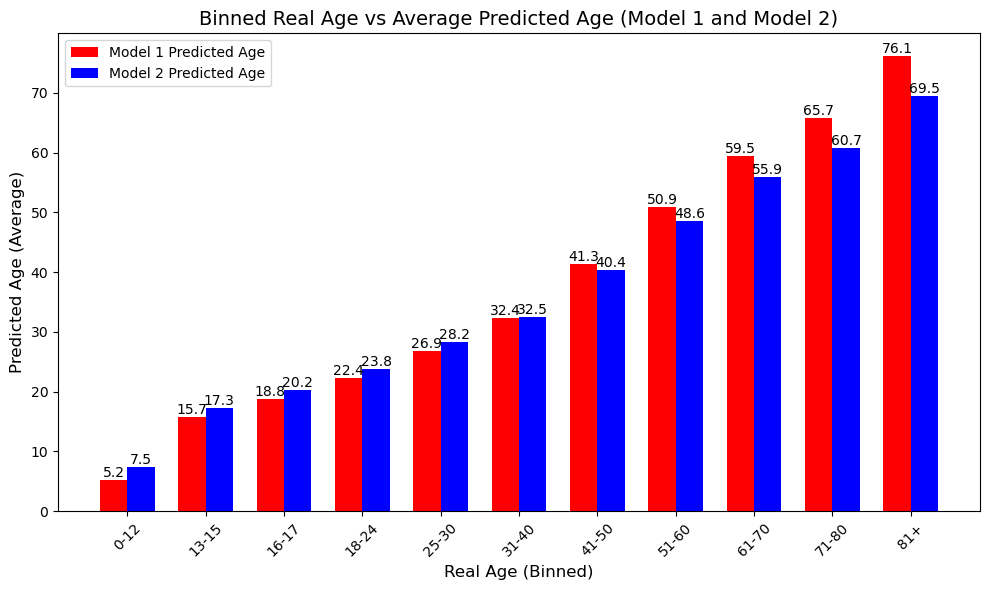
\includegraphics[width=\textwidth]{images/2_Bars_Real_vs_prediction_dorpnan.png}
        \caption{Bar plot comparing the average prediction of both models at each real-age bracket.}
        \label{fig:Bar}
    \end{minipage}
\end{figure}

%When observing Figure~\ref{fig:Bar}:
%\begin{table}[h]
%\centering
%\begin{tabular}{l|c|c}
%\hline
%\textbf{Age Bin} & \textbf{Model 1} & \textbf{Model 2} \\ \hline
%0-12   & Good    & Good \\ 
%13-15  & Bad     & Bad  \\    
%16-17  & Bad     & Bad  \\     
%18-24  & Good    & Good \\      
%25-30  & Good    & Good \\      
%31-40  & Good    & Good \\      
%41-50  & Good    & God  \\     
%51-60  & Good    & Bad  \\     
%61-70  & Good    & Bad  \\     
%71-80  & Bad     & Bad  \\     
%81+    & Bad     & Bad      \\ \hline
%\end{tabular}
%\caption{Comparison of Model 1 and Model 2 predictions across different age bins.}
%\label{tab:comparison}
%\end{table}




\begin{figure}[h]
    \centering
    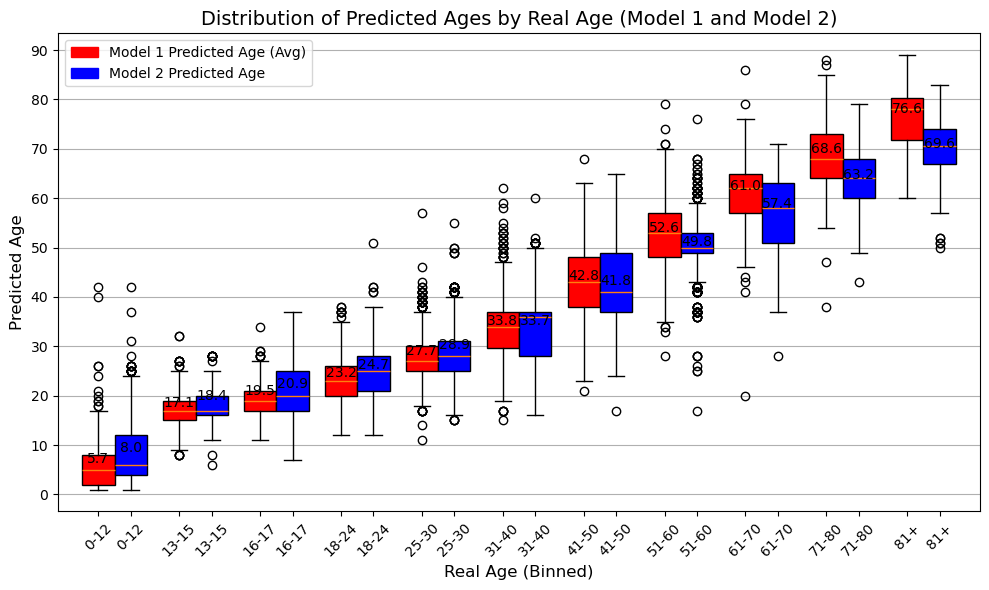
\includegraphics[width=0.8\textwidth]{images/3_Box_Real_vs_prediction_dorpnan_DensePlotGrid.png}
    \caption{Caption describing the image.}
    \label{fig:Box}
\end{figure}

\section{Conclusion}
(Here, you'd summarize findings and suggest which model is preferable based on performance metrics.)

\end{document}
